\chapter{La notación asintótica}

\begin{marginfigure}
  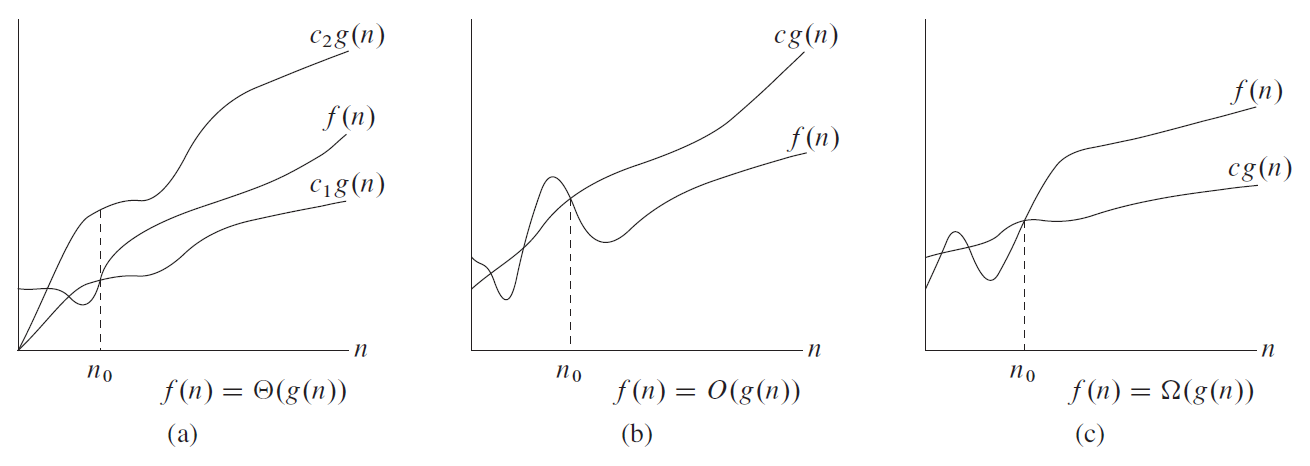
\includegraphics[width=\linewidth]{figuras/big-o}
  \caption{Interpretación gráfica de la notación asintótica. La notación \(f=O(g)\) implica que \(g\) es una cota superior para \(f\).}
\end{marginfigure}

\begin{marginfigure}
  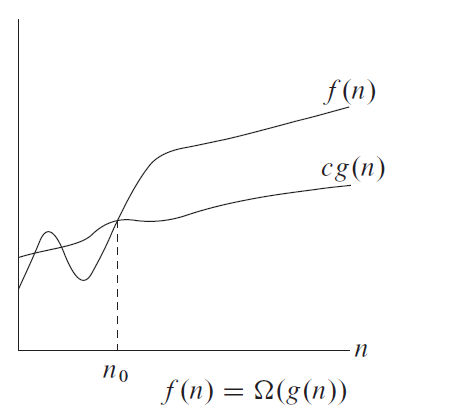
\includegraphics[width=\linewidth]{figuras/big-omega}
  \caption{La notación \(f=\Omega(g)\) implica que \(g\) es una cota inferior para \(f\).}
\end{marginfigure}

\begin{marginfigure}
  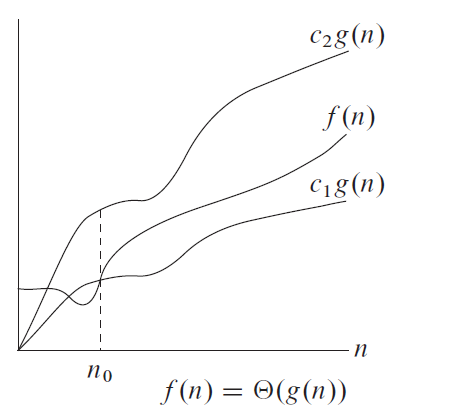
\includegraphics[width=\linewidth]{figuras/big-theta}
  \caption{La notación \(f=\Theta(g)\) implica que \(g\) es una cota ajustada para \(f\).}
\end{marginfigure}

La \emph{notación asintótica} (también conocida como la \emph{notación de Landau}) es una notación matemática que se utiliza para caracterizar la tasa de crecimiento de una función con respecto a otra cuando la variable independiente crece infinitamente.
La noción básica de esta notación es que, dada una expresión algebraica, los términos de mayor grado crecen más rápido que aquellos de menor grado y, por ende, el efecto que estos últimos tienen sobre la tasa de crecimiento de la expresión es despreciable cuando la variable independiente crece infinitamente. 
En el análisis de la eficiencia de un algoritmo, la notación asintótica se utiliza para describir el tiempo de ejecución del algoritmo o para comprar dos algoritmos en términos de su respectiva eficiencia.

\section{Definiciones}

Sea $n\in\mathbb{N}$ y sean $f:\mathbb{N}\to\mathbb{R}$ y $g:\mathbb{N}\to\mathbb{R}$
dos funciones \emph{asintóticamente no-negativas} (i.e. $f(n)$ y $g(n)$
siempre son no-negativos a partir de algún valor determinado de $n$), a continuación
se presentan las definiciones básicas para la notación asintótica. Obsérvese que, en 
esta notación, se utiliza el símbolo $=$, en lugar de 
$\in$, para denotar la pertenencia a alguno de los conjuntos introducidos.

\begin{defn}[O grande]
    Denotado como $O(g)$, es el conjunto de todas aquellas funciones
    $f$ para las cuales existen dos constantes $c\in\mathbb{R}$ y $n_{0}\in\mathbb{N}$
    tales que $0\le f(n)\leq c g(n)$, para toda $n\geq n_{0}$. 
\end{defn}

\begin{defn}[$\Omega$ grande]
    Denotado como $\Omega(g)$, es el conjunto de todas aquellas funciones
    $f$ para las cuales existen dos constantes $c$ y $n_{0}$ tales
    que $0\le c g(n)\leq f(n)$, para toda $n\geq n_{0}$.
\end{defn}

\begin{defn}[$\Theta$ grande]
    Denotado como $\Theta(g)$, es el conjunto de todas aquellas funciones
    $f$ para las cuales existen tres constantes $c_{1},c_{2}\in\mathbb{R}$
    y $n_{0}$ tales que $0\le c_{1} g(n)\leq f(n)\leq c_{2} g(n)$,
    para toda $n\geq n_{0}$.
\end{defn}

\begin{prop}
    Se tiene que $f=\Theta(g)$ si y sólo si $f=O(g)$ y $f=\Omega(g)$.
\end{prop}

\begin{defn}[o chica]
    Denotado como $o(g)$, es el conjunto de todas aquellas funciones
    $f$ tales que, para toda constante $c$, existe una constante $n_{0}$
    tal que $0\leq f(n)<c g(n)$ para toda $n\geq n_{0}$.
\end{defn}

\begin{defn}[$\omega$ chica]
    Denotado como $\omega(g)$, es el conjunto de todas aquellas funciones
    $f$ tales que, para toda constante $c$, existe una constante $n_{0}$
    tal que $0\leq c g(n)<f(n)$ para toda $n\geq n_{0}$.
\end{defn}

\begin{prop}
    Si $f=o(g)$, entonces $f=O(g)$.
\end{prop}

\begin{prop}
    Si $f=\omega(g)$, entonces $f=\Omega(g)$.
\end{prop}

La notación asintótica también se puede definir en términos del límite
de la razón de las funciones involucradas (suponiendo que dicho límite
existe). 

\begin{prop}
    Se tiene que
    
    \[
        \lim_{n\to\infty}\dfrac{f(n)}{g(n)}\in\begin{cases}
            [0,\infty) & \text{si y sólo si }f=O(g)\\
            (0,\infty] & \text{si y sólo si }f=\Omega(g)\\
            (0,\infty) & \text{si y sólo si }f=\Theta(g)
        \end{cases}
    \]
\end{prop}

\begin{prop}
    Se tiene que

    \[
        \text{si }\lim_{n\to\infty}\dfrac{f(n)}{g(n)}=\begin{cases}
        0 & \text{entonces }f=o(g)\\
        \infty & \text{entonces }f=\omega(g)\\
        1 & \text{entonces }f\sim g
        \end{cases}
    \]
\end{prop}

\begin{prop}
    Si $f\sim g$, entonces $f=\Theta(g)$.
\end{prop}

\section{La notación asintótica y el símbolo de igualdad}

Como se mencionó anteriormente, en la notación asintótica se utiliza
$=$ para denotar que una función determinada pertenece a alguno de los conjuntos
introducidos. Este abuso de notación se permite por razones que se 
vuelven aparentes en esta sección.

Cuando la notación asintótica se utiliza dentro de alguna expresión algebraica, dicha 
notación se interpreta como que representa alguna función anónima perteneciente
al conjunto correspondiente.

Cuando la notación asintótica aparece en ambos lados de una ecuación, entonces
la notación se interpreta de la sig. manera: \emph{sin importar cómo se elijan las 
funciones anónimas del lado izquierdo de la ecuación, siempre hay una manera de elegir 
las funciones anónimas del lado derecho de tal forma que la ecuación se cumple}.
Por ejemplo, si se tiene $2n^2+\Theta(n)=\Theta(n^2)$, esto quiere decir que,
para cualquier $f\in\Theta(n)$, hay una $g\in\Theta(n^2)$ tal que $2n^2+f(n)=g(n)$ 
se cumple para toda $n$.

Cuando se escriben tres o más ecuaciones de forma encadenada, cada par de expresiones
en la cadena se pueden interpretar independientemente utilizando las dos reglas anteriores,
por ejemplo, cuando se tiene $2n^2+3n+1=2n^2+\Theta(n)=\Theta(n^2)$, que implica que
$2n^2+3n+1=\Theta(n^2)$; i.e. que $2n^2+3n+1\in\Theta(n^2)$.

\section{Propiedades aritméticas de la notación asintótica}

La suma de las cotas de dos funciones está gobernada por la función
dominante. Esto es:

\[
\begin{aligned}
    O(f)+O(g) &= O(\max\{f,g\})\\
    \Omega(f)+\Omega(g) &= \Omega(\max\{f,g\})\\
    \Theta(f)+\Theta(g) &= \Theta(\max\{f,g\})
\end{aligned}
\qquad
\begin{aligned}
    o(f)+o(g) &= o(\max\{f,g\})\\
    \omega(f)+\omega(g) &= \omega(\max\{f,g\})
\end{aligned}
\]

La multiplicación entre una función y una constante no afecta el
comportamiento asintótico de dicha función. Esto es:

\[
\begin{aligned}
    O(c\cdot f) &= O(f)\\
    \Omega(c\cdot f) &= \Omega(f)\\
    \Theta(c\cdot f) &= \Theta(f)
\end{aligned}
\qquad
\begin{aligned}
    o(c\cdot f) &= o(f)\\
    \omega(c\cdot f) &= \omega(f)
\end{aligned}
\]

Cuando dos funciones se multiplican, ambas contribuyen por igual al
comportamiento asintótico de la función resultante. Esto es:

\[
\begin{aligned}
    O(f)\cdot O(g) &= O(f\cdot g)\\
    \Omega(f)\cdot\Omega(g) &= \Omega(f\cdot g)\\
    \Theta(f)\cdot\Theta(g) &= \Theta(f\cdot g)
\end{aligned}
\qquad
\begin{aligned}
    o(f)\cdot o(g) &= o(f\cdot g)\\
    \omega(f)\cdot\omega(g) &= \omega(f\cdot g)
\end{aligned}
\]

La notación asintótica también se puede utilizar como un esquema para comparar
dos funciones y decidir cuál crece más rápido. Una
forma intuitiva de verlo es trazando las analogías mostradas en la 
Tabla \ref{tab:func-comp}. Esto es posible gracias a que muchas de 
las propiedades de relación de los números reales también aplican en la
notación asintótica. Estas propiedades se describen a continuación y
suponen que $f$ y $g$ son \emph{asintóticamente positivas}.

\begin{table}
\label{tab:func-comp}
\caption{Operaciones de comparación de números reales y su funcionamiento análogo en 
notación asintótica.}
\centering
\begin{tabular}{cc}
    \toprule 
        Números reales & Notación asintótica\tabularnewline
    \midrule
        $a\leq b$ & $f=O(g)$\tabularnewline
        $a\ge b$ & $f=\Omega(g)$\tabularnewline
        $a=b$ & $f=\Theta(g)$\tabularnewline
        $a<b$ & $f=o(g)$\tabularnewline
        $a>b$ & $f=\omega(g)$\tabularnewline
    \bottomrule
\end{tabular}
\end{table}

Todos los conjuntos de la notación asintótica poseen la propiedad de transitividad.
Esto es, sea $h:\mathbb{N}\to\mathbb{R}$ una función asintóticamente positiva, se
tiene que:

\begin{itemize}[label=\textbullet]
    \item Si $f=\Theta(g)$ y $g=\Theta(h)$, entonces $f=\Theta(h)$.
    \item Si $f=O(g)$ y $g=O(h)$, entonces $f=O(h)$. 
    \item Si $f=\Omega(g)$ y $g=\Omega(h)$, entonces $f=\Omega(h)$.
    \item Si $f=o(g)$ y $g=o(h)$, entonces $f=o(h)$.
    \item Si $f=\omega(g)$ y $g=\omega(h)$, entonces $f=\omega(h)$.
\end{itemize}

Algunos conjuntos poseen la propiedad de reflexividad. Esto es: 
$f=\Theta(f)$, $f=O(f)$ y $f=\Omega(f)$. 
Lo anterior se cumple porque $f(n)=f(n)$ para toda $n$.

El conjunto $\Theta$ grande posee la propiedad de simetría y algunos conjuntos 
poseen la propiedad de simetría traspuesta. Esto es:

\marginnote{Cabe mencionar que, dado que $\Theta$ grande posee las propiedades de 
reflexividad, transitividad y simetría, este conjunto es, de hecho, una relación de 
equivalencia.}

\begin{itemize}[label=\textbullet]
    \item $f=\Theta(g)$ si y sólo si $g=\Theta(f)$.
    \item $f=O(g)$ si y sólo si $g=\Omega(f)$.
    \item $f=o(g)$ si y sólo si $g=\omega(f)$.
\end{itemize}

Por último, la notación asintótica carece de la propiedad
de tricotomía, que es la propiedad de los números reales donde, dados dos
números $a$ y $b$, siempre se cumple exactamente una de las sig.
posibilidades: $a<b$, $a=b$ o $a>b$. La notación asintótica carece
de esta propiedad porque se puede dar el caso donde no se cumple
que $f=O(g)$ ni que $f=\Omega(g)$ (para alguna $n$ suficientemente grande).
Por ejemplo, si se tiene que
$f(n)=n$ y $g(n)=n^{1+\sin{n}}$, el comportamiento 
asintótico de estas funciones no se puede comparar porque el
exponente $1+\sin{n}$ oscila entre 0 y 2, tomando todos los
valores intermedios.

\section{Ordenes de crecimiento de uso frecuente}

A continuación se presentan los órdenes
de crecimiento que se observan con mayor frecuencia en las ciencias de la
computación, listados de aquél que crece más lento
al que crece más rápido.

\begin{enumerate}
\begin{multicols}{2}
    \item \emph{Constantes}: $O(1)$
    \item \emph{Logarítmicos}: $O(\log n)$
    \item \emph{Radicales}: $O(\sqrt{n})$
    \item \emph{Lineales}: $O(n)$
    \item \emph{Súper lineales}: $O(n\log n)$
    \item \emph{Cuadráticos}: $O(n^{2})$
    \item \emph{Cúbicos}: $O(n^{3})$
    \item \emph{Exponenciales}: $O(2^{n})$
    \item \emph{Factoriales}: $O(n!)$
\end{multicols}
\end{enumerate}

Se debe tener cuidado sobre cómo interpretar la lista anterior, ya
que la notación asintótica puede ocultar constantes muy grandes y 
dejar una impresión equivocada de la tasa de crecimiento
de una función comparada con otra. 
Por ejemplo, supóngase que se tiene que $f(n)=10^{100}n=O(n)$
y que $g(n)=10n\cdot\log n=O(n\log n)$. A pesar de que la notación
asintótica indica que $g$ crece más rápido que $f$, en realidad
se trata de lo opuesto, porque la constante $10^{100}$ supera por mucho 
la tasa de crecimiento de $g$.

\begin{thm}
    Sea $k\in\mathbb{N}_{0}$ una constante. Todo polinomio de grado $k$
    pertenece a $\Theta(n^{k})$.
\end{thm}

\begin{proof}
    Sea $f(n)=a_{k}n^{k}+a_{k-1}n^{k-1}+\dots+a_{1}n+a_{0}$ un polinomio
    arbitrario, donde $a_k,\dots,a_{0}\in\mathbb{R}$ son constantes.
    Por la definición de $\Theta$ grande, se requiere demostrar que $f=O(n^{k})$
    y que $f=\Omega(n^{k})$. 
    
    Para demostrar que $f=O(n^{k})$, se tiene que 
    
    \begin{align*}
        a_{k}n^{k}+a_{k-1}n^{k-1}+\dots+a_{1}n+a_{0} &=\\ n^{k}(a_{k}+a_{k-1}/n+\dots+a_{1}/n^{k-1}+a_{0}/n^{k}) &\leq\\
        n^{k}(a_{k}+a_{k-1}+\dots+a_{1}+a_{0})
    \end{align*}
    lo que se cumple para toda $n\geq1$. Por lo tanto, $f=O(n^{k})$.
    
    Para demostrar que $f=\Omega(n^{k})$, se tiene que 
    
    \[
        n^{k}(a_{k}+a_{k-1}/n+\dots+a_{1}/n^{k-1}+a_{0}/n^{k})\geq n^{k}
    \]
    lo que se cumple para toda $n\geq1$. Por lo tanto, $f=\Omega(n^{k})$.
\end{proof}

\begin{thm}
    Toda función polinomial crece más rápido que cualquier función logarítmica y
    toda función exponencial crece más rápido que cualquier función polinomial.
    Esto es, sean $k,q\in\mathbb{N}$ constantes, se tiene que $(\log n)^k=o(n^q)$
    y $n^k=o(q^n)$.
\end{thm}

\begin{proof}
    Ambas relaciones se pueden demostrar utilizando límites y la regla
    de L'Hopital. Así, para la primera expresión, se tiene que
    
    \begin{align*}
        \lim_{n\to\infty}\dfrac{(\ln n)^{k}}{n^{q}} &= \left(\lim_{n\to\infty}\dfrac{\ln n}{n^{q/k}}\right)^{k}\\
        &\overset{\text{H}}{=}\left(\lim_{n\to\infty}\dfrac{1/n}{(q/k)n^{q/k-1}}\right)^{k}\\
        &= \left(\lim_{n\to\infty}\dfrac{1}{(q/k)n^{q/k}}\right)^{k}\\
        &= 0
    \end{align*}
    Por lo tanto, $(\log n)^{k}=o(n^{q})$.
    
    Para la segunda expresión, se tiene que 
    
    \begin{align*}
    \lim_{n\to\infty}\dfrac{n^{k}}{q^{n}} &= \left(\lim_{n\to\infty}\dfrac{n}{q^{n/k}}\right)^{k}\\
    &\overset{\text{H}}{=}\left(\lim_{n\to\infty}\dfrac{1}{(n/k)q^{n/k-1}}\right)^{k}\\
    &= 0
    \end{align*}
    Por lo tanto, $n^{k}=o(q^{n})$.
\end{proof}

\section*{Referencias}

\begin{itemize}[label=\textbullet]
    \item \fullcite[43--52]{cormen_2009}.
    \item \fullcite[34--41]{skiena_2011}.
    \item \fullcite[13--20]{goodrich_2001}.
    \item \fullcite[20--23]{mcconnell_2001}.
    \item \fullcite{baker_2013}
    \item \fullcite{leighton_2004}
    \item \fullcite{tomescu_2014}
\end{itemize}